% --------------------------------------------------------------------

\section{Johdanto}

Ohjelmistoprojekteissa tulee väistämättä vastaan ongelmia. Näiden järjestelmällinen analysointi ja ehkäiseminen jatkuvana osana kehitysprosessia parantaa ohjelmistoprojektin mahdollisuuksia onnistua. Ketterässä ohjelmistokehityksessä kehitystiimi järjestää säännöllisesti reflektion, jossa tiimi tarkastelee työtapojaan ja tiimityöskentelyään, sekä pohtii tapoja, joilla voi sopeuttaa niitä päästäkseen parempiin tuloksiin \citep{AgileRetros2006}. Kehitystiimi pyrkii tutkimaan konkreettisia ongelmia ja löytämään niihin konkreettisia ratkaisuja \citep{AgileRetros2006}. Juurisyyanalyysi (RCA, Root Cause Analysis) tarjoaa rakenteellisen tavan löytää ongelmien aiheuttajia ja voi siten auttaa ehkäisemään näiden ongelmien esiintymistä jatkossa \citep{Lehtinen2011}. Rakenteellinen tapa tunnistaa ongelmien aiheuttajia sopii hyvin retrospektiivin ongelmanratkaisuun (tähän viite esim ESEM paperiin). Juurisyyanalyysiä voi kuitenkin tehdä lukuisalla eri tavalla \citep{Lehtinen2011}.

Vaikka iteraation lopussa pidettävä retrospektiivi on olennainen osa ketterän ohjelmistokehitysprosessin runkoa, ei sen toteutustapavasta ole yhteistä käytäntöä. Retrospektiivin järjestäminen on määritelty ketterien menetelmien yleisissä periaatteissa \citep{AgileManifestoPrinciples}. Retrospektiivin tavoitteet saattavat olla määritelty tarkasti noudatettavan ketterän ohjelmistokehitysmetodologian kuvauksessa, mutta sen toteutustapa on usein jätetty yleensä tiimin päätettäväksi. Esimerkiksi Scrum-metodologian kuvauksessa on kuvattu retrospektiivien tavoitteet, muttei niiden saavuttamiseen johtavia menetelmiä \citep{ScrumGuide2011}.

Tässä kandidaatintyössä tutkitaan systemaattisen kirjallisuuskatsauksen \citep{Kitchenham2010} avulla juurisyyanalyysiä soveltavia retrospektiivejä. Työssä vastataan seuraaviin tutkimuskysymyksiin:
\begin{enumerate}
\item Minkälaisia menetelmiä aiemmassa kirjallisuudessa on esitetty juurisyyanalyysiä soveltaviin retrospektiiveihin?
\item Minkälainen menetelmä voisi sopia ketterän ohjelmistokehitystiimin retrospektiiviin?
\end{enumerate}
Menetelmän tulee olla kevyt ja yksinkertainen toteuttaa, jotta sen käyttöönotto lyhyehköissä iteraatio-retrospektiiveissä olisi mielekästä. Esimerkiksi extreme programming -metodologiaan on suositeltu lyhyitä ja tehokkaita retrospektiivejä, jotka eivät vaadi kovin suurta panosta tiimiltä, mutta tuottavat siitä huolimatta välittömiä ja näkyviä tuloksia \citep{myllyaho2004review}. Aineistohaut rajoitettiin Scopus-tietokannan tieteellisiin artikkeleihin.

Tämä kandidaatintyö on jaettu seuraaviin osiin. Kappaleessa 2 esitellään teoreettinen tausta, joka sisältää määritelmät ketterälle retrospektiiville ja juurisyyanalyysille. Kappaleessa 3 kuvataan työssä käytetyt tutkimusmenetelmät. Kappaleessa 4 tuodaan julki tulokset ja kappaleessa 5 tulosten johtopäätösket ja niihin liittyvät validiteettiuhat. Kandidaatintyön viimeinen kappale on yhteenveto.

\section{Teoreettinen tausta}

\subsection{Ketterä retrospektiivi}
Tässä työssä retrospektiivillä tarkoitetaan... TODO!
Ketterissä ohjelmistokehitysmenetelmissä on määritelty, että säännöllisin väliajoin pidetään reflektointi, jossa kehitystiimi pohtii tapoja tulla tehokkaammaksi. Kehitettyjen parannusehdotusten perusteella tiimi muuttaa toimintaansa \citep{AgileManifestoPrinciples}. Kevyt retrospektiivisessio on tapa toteuttaa tätä reflektointia \citep{Cockburn2002}i. Projektin lopputuloksen kannalta retrospektiivejä on järkevää pitää lyhyin väliajoin \citep{Cockburn2002}. Tällöin tiimin kohtaamat ongelmat ja niihin liittyvät yksityiskohdat ovat tuoreessa muistissa ja parannusehdotukset voidaan ottaa suoraan käyttöön ja siten pyrkiä parantamaan projektin lopputuloksen laatua \citep{Cockburn2002}.

XP- ja Scrum-metodologiassa retrospektiivejä suositellaan pidettäväksi joka iteraation päätteeksi \citep{Lindstrom2004, ScrumGuide2011}. Iteraatiolla tarkoitetaan ketterissä ohjelmistokehitysmenetelmissä suosittuja lyhyitä kehityssyklejä, joihin ohjelmointityö on jaettu \citep{beck1999embracing}. Iteraation voi mieltää pieneksi, enintään kuukauden pituiseksi projektiksi \citep{ScrumGuide2011}  Iteraatioretrospektiiveissä kehitystiimi reflektoi sitä, missä he ovat viime iteraation aikana onnistuneet hyvin ja missä on vielä kehitettävää \citep{Lindstrom2004, ScrumGuide2011}. Retrospektiivin avulla tiimi saa palautetta työstään \citep{Lindstrom2004}. Retrospektiivissä voidaan muun muassa pohtia sitä, miten kurinalaisesti kehitystiimi on noudattanut työkäytäntöjä ja voisiko niitä räätälöidä sopimaan paremmin tiimin tarpeisiin \citep{Lindstrom2004}.

\subsection{Juurisyyanalyysi}
Juurisyyanalyysi on rakenteellinen tapa tutkia ongelmia ja tunnistaa niiden aiheuttajia \citep{Lehtinen2011}. Juurisyyanalyysi pohjautuu teoriaan, jonka mukaan ongelman uudelleenesiintyminen voidaan välttää kontrolloimalla sen aiheuttajia \citep{Lehtinen2011}. Juurisyyanalyysin avulla voidaan tutkia ongelmien lisäksi myös onnistumisten syitä. \citep{Bjornson2009} Juurisyylle on useita määritelmiä \citep{Lehtinen2011}. Se voi tarkoittaa mitä tahansa ongelman aiheuttavaa syytä, syyketjun perimmäisintä syytä tai syytä, johon johto voi vaikuttaa \citep{Lehtinen2011}. Juurisyyanalyysin tuloksia voidaan käyttää apuna prosessinkehityksessä. \citep{Lehtinen2011}

\section{Systemaattinen kirjallisuuskatsaus tutkimusmenetelmänä}

\subsection{Taustaa}
Systemaattisessa kirjallisuuskatsauksessa (SLR, Systematic Literature Review) tehdään kattava arviointi valitusta aiheesta. Arvioinnissa käytetään luotettavaa, tarkkaa ja toistettavisaa olevaa menetelmää. SLR on kirjallisuuskatsauksen muoto, mikä tarkoittaa sitä, että siinä käydään läpi aiempia tutkimuksia, jotka ovat olennaisia työssä esitettävien tutkimuskysymysten kannalta. Kerätyn kirjallisuuden pohjalta muodostetaan synteesi, eli kerätään, yhdistetään ja tehdään yhteenveto kerätystä aineistosta. \citep{Kitchenham2007}

SLR:n erityispiirteenä on se, että kirjallisuuden etsiminen, valikointi ja valitun kirjallisuuden analysointi pyritään tekemään toistettavasti ja puolueettomasti. Kitchenham perustelee SLR-menetelmän hyötyä toteamalla, että kirjallisuuskatsaus, joka ei ole SLR:n tapaan perusteellinen ja tasapuolinen ei tarjoa paljoa tieteellistä arvoa. Systemaattisen kirjallisuuskatsauksen tulokset ovat todennäköisemmin puolueettomia, eli tutkijan kannasta riippumattomia. \citep{Kitchenham2007}

Systemaattinen kirjallisuuskatsaus koostuu kolmesta päävaiheesta: suunnittelu-, toteutus- ja raportointivaiheista. Suunnitteluvaiheessa tunnistetaan kirjallisuuskatsauksen tarve, määritellään tutkimuskysymykset, sekä protokolla katsauksen suorittamiselle. \citep{Kitchenham2007}

Toteutusvaiheessa tehdään aineistohakuja ja valitaan ennaltamääritellyin kriteerein tutkimukselle olennaiset artikkelit. Artikkelien laatua ja sitä kautta luotettavuutta arvioidaan. Tehdyistä hauista kirjataan kaikki kirjallisuuskatsauksen toistamiseen ja sen laadun arviointiin tarvittava tieto, kuten haussa käytetyt hakukoneet, hakusanat, löydettyjen tulosten määrä ja jopa tuloslista. Valitusta aineistosta kerätään tietoa talteen ja sen merkittävyyttä omalle tutkimukselle arvioidaan ennalta määritellyin kriteerein. Kerätyn ja merkittäväksi valitun tiedon perusteella muodostetaan synteesi. Raportointivaiheessa kirjoitetaan tulokset ylös ja arvioidaan tuloksia. \citep{Kitchenham2007}

Tähän kandidaatintyöhön valittiin Kitchenhamin määrittelemä systemaattinen kirjallisuuskatsaus, jotta kerätty aineistolista ja sen pohjalta saadut tulokset olisivat tieteellisesti merkittävämpiä, sekä mahdollisesti myös muulle tutkimukselle käyttökelpoisia.

\subsection{Rajaukset}
Haettavan aineiston olennaisin rajaus on määrittää, minkälainen sisältö on tämän työn kannalta merkittävää. Aineiston tulisi vastata työn tutkimuskysymykseen, eli siihen, minkälaisia menetelmiä aiemmassa kirjallisuudessa on esitetty juurisyyanalyysiä soveltaviin retrospektiiveihin.

Ennen kirjallisuuskatsauksen aloittamista kandidaatintyön ohjaajan kanssa sovittiin seuraavat rajaukset. Aineistohaut suoritettaisiin pelkästään Scopus-tietokantaan. Haku rajataan pelkkiin tieteellisiin artikkeleihin. Haetut artikkelit eivät saa olla julkaistu ennen vuotta 1990. Myös käytettävät hakusanat sovittiin alustavati kattamaan sanat "retrospective",  "postmortem analysis", "post-project review" ja "software engineering". Näistä hakusanoista tulisi kokeilla erilaisia yhdistelmiä.

Rajaukset tehtiin, jotta kandidaatintyön työmäärä pysyisi järkevänä. Seuraavaksi käydään läpi yksittäisten rajausten perustelut. Scopus-tietokanta valittiin kandidaatintyön ohjaajan suosituksesta. Haku rajattiin tieteellisiin artikkeleihin, jotta työn tulokset pohjautuisivat objektiiviseen tutkimustietoon. Vuosi 1990 valittiin, koska samana vuonna on julkaistu teos \citep{ishikawa1990introduction}, jokna myötä RCA on alkanut vakiintua. Hakusanat valitiin sisältämään eri nimityksiä retrospektiiveille, joita on retrospektiivin lisäksi muun muassa "post-mortem analysis" ja "post project review". Nämä ovat yleensä projektitasolla järjestettyjä retrospektiivejä. Ohjelmistotuotanto ("software engineering") valittiin hakusanaksi rajaamaan haku kattamaan ainoastaan ohjelmistotuotannon alan retrospektiivit.

Ajatuksena oli tehdä haku retrospektiivin näkökulmasta ja löytää sieltä viitteitä juurisyyanalyysin käytöstä. Näin ollen "juurisyyanalyysi" ei kuulunut hakusanoihin, vaan sitä etsittäisiin löydetystä aineistosta. Kirjallisuuskatsauksen tavoitteena oli käsitellä retrospektiiveihin liittyvät tieteelliset artikkelit, joissa esitellään juurisyyanalyysiä soveltavat retrospektiivimenetelmät 1990 luvulta lähtien.

\subsection{Hakutermin muodostuminen}
TODO: tähän jäin timon korjauksissa
Kandidaatintyön kirjoittaja aloitti systemaattisen kirjallisuuskatsauksen kokeilemalla erilaisia yhdistelmiä määritellyistä hakusanoista ja hakemalla niitä eri tavoin artikkeleista. Tavoitteena oli löytää mahdollisimman kattava kuva rajatusta kokonaisuudesta. Aineistohaulla tulisi löytää riittävä määrä artikkeleita, jotta kirjallisuuskatsauksen otos ei olisi liian suppea ja saattaisi tutkimuksen luotettavuuden sen takia kyseenalaiseksi. Kuitenkin artikkelien määrän tulee olla järkevästi käsiteltävissä kandidaatintyön määrittämän työmäärän puitteissa. Kandidaatintyön tekijä sopi yhdessä työn ohjaajan kanssa sopivan otoskoon olevan noin 100 artikkelia. Haun tulosten arvioinnissa hyödynnettiin ohjaajan jo aiemmin löytämiä relevantteja artikkeleita, kuten \citep{Bjornson2009} ja \citep{card1998learning}. Hakutermejä laajennettiin niin kauan kunnes kaikki jo aiemmin löydetyt relevantit artikkelit löytyivät hakutermeillä ja hakutermit näyttivät muutenkin pintapuolisella tarkastelulla järkeviltä. Tämä johti lopulta 108 artikkelin kattavaan joukkoon.

Alkuperäinen suunnitelma oli käyttää pelkästään hakusanoja "retrospective",  "postmortem analysis", "post-project review" ja "software engineering". Kuitenkin, koska näillä hakusanoilla olennaisten hakutulosten lukumäärä osoittautui liian pieneksi, otettiin hakusanoiksi mukaan juurisyyanalyysiä kuvaavat hakusanat: "root cause analysis", "rca", "defect cause analysis" ja "dca". Alunperin oli siis tarkoitus etsiä mainintaa juurisyyanalyysin käytöstä retrospektiivin menetelmänä retrospektiiviä kuvaavista artikkeleista. Valittujen uusien hakusanojen myötä haetiin nyt lisäksi retrospektiiviä että juurisyyanalyysiä käsittelevistä artikkeleista. Siten kandidaatintyön aihetta lähestyttiin ikään kahdelta suunnalta: erikseen retrospektiivin ja juurisyyanalyysin näkökulmista.

Hakusana "software engineering" osoittautui niin yleiseksi ja lähinnä aihealuetta kuvaavaksi, etteivät artikkelit yleensä maininneet sitä otsikossaan, abstraktissa tai artikkelin avainsanoissa. Siksi haemme kyseistä hakusanaa kaikista mahdollisista hakukentistä, eikä pelkästään edellämainituista kolmesta. Lisäksi käytämme Scopuksen omaa aihealuerajausta ja haemme ainoastaan artikkeleja tietotekniikan aihealueelta.

Lopulliseksi hakutermiksi muodostui seuraava:\\
\textit{ALL("software engineering") AND TITLE-ABS-KEY("retrospective" OR "postmortem analysis" OR "pma" OR "post-mortem" OR "post mortem analysis" OR "post-project review" OR "post project review" OR "root cause analysis" OR "rca" OR "defect cause analysis" OR "dca") AND DOCTYPE(ar) AND SUBJAREA(comp) AND PUBYEAR > 1989}\\
Näillä hakusanoilla löytyi yhteensä 108 tulosta.

Kirjallisuuskatsauksessa käytettyjen hakusanojen evoluutio erilaisine kokeiluineen ja niiden toimivuuden arvioinnin kera on kuvattu kandidaatin työn liitteessä \ref{sec:hakutermi_evoluutio}.

\subsection{Tulosten arviointi}
Haun tulokset tallennettiin taulukkolaskentaohjelmaan. Kaikki 108:n artikkelin abstraktit luettiin. Tuloksia arvioitiin eri tavoin käyttämällä artikkelin otsikon, abstraktin ja avainsanojen antamia tietoja. Artikkeleista merkittiin ylös sisältävätkö ne retrospektiivimenetelmän kuvauksen, juurisyyanalyysin, jonkin retrospektiivissä käytettävän menetelmän, ja sisältääkö kuvattu retrospektiivin menetelmä juurisyyanalyysin. Lisäksi merkittiin ylös, kuvataanko artikkelissa ketteriä menetelmiä ja nimenomaan ketterää retrospektiiviä. Artikkeleista kirjoitettiin taulukkolaskentaohjelmaan myös lyhyet muistiinpanot.

Tulosten rajausvaiheessa artikkeleista merkittiin vielä kuvaavatko ne prosessinkehitystä ja onko kuvattu retrospektiivi kollaboratiivinen sessio yrityksen työntekijöiden (esim kehitystiimin) välinen sessio (eikä esim tutkijoiden jälkeenpäin suorittama). Näillä lisämerkinnöillä helpotettiin artikkelien rajaamista. Nämä merkinnät tehtiin pääosin taulukkolaskentaohjelmaan tehtyjen muistiinpanojen perusteella. Epäselvissä tapauksissa abstrakti luettiin uudestaan, tai  aineistolistaan artikkelin kohdalle merkittiin kysymysmerkki, mikäli asia ei selvinnyt siitä.

Jokaiseen ylläkuvatuista kysymyksistä (merkitty sarakkeina taulukkolaskentaohjelmassa) merkittiin "kyllä" tai "ei". Epäselvissä tapauksissa merkittiin kysymysmerkki, "ehkä", tai kohta saatettiin jättää tyhjäksi. Näitä kahta merkintää käytettiin kandidaatintyön tekijän oman tuntuman mukaan. Merkintää "ehkä" käytettiin silloin, kun kriteerin täyttyminen oli todennäköisempää ja kysymysmerkkiä, kun sen se oli epätodennäköisempää. 

Oli myös tapauksia, joissa artikkeli ei täysin täyttänyt kohdan kriteerejä, esimerkiksi sisälsi jonkin retrospektiivin tapaisen lähestymistavan, jota ei kuitenkaan voinut aivan mieltää retrospektiiviksi. Tällainen oli esimerkiksi artikkeli \citep{cook1998cost}, joka tutki yrityksen prosessin kehittämistä vanhoja prosessien ja tuotteiden dokumentaatioita hyödyntämällä. Tämä menetelmä on tavallaan retrospektiiviä siinä mielessä, että siinä pyritään kehittämään yrityksen prosessia tarkastelemalla vanhoja tapahtumia. Kuitenkaan se ei tuntunut kuvaavan retrospektiivi-tapahtumaa, jossa yrityksen edustajia kokoontuu ja aktiivisesti pohtii menneen työrupeaman onnistumisia ja epäonnistumisia. Tämäntyyppisten artikkelien kohdalla aineistolistaan merkittiin artikkelin tietyn kriteerin kohdalle "sinne päin". 

\subsection{Tulosten rajaus}
Taulukossa \ref{tab:karsintaehdot_taulukko} on esitetty perusteet, joiden mukaan tuloksia on karsittu pois. Karsinta on tehty edellä kuvattujen arviointien perusteella. Ensimmäinen haku Scopus-hakukoneessa tehtiin 26. maaliskuuta 2013, jolloin artikkeleja löytyi 108. Seuraavana päivänä artikkeleja löytyi enää 106. Kaksi hausta pudonnutta artikkelia olivat \citep{bolosky2007farsite} ja \citep{dreiseitl2005nomographic}. Nämä artikkelit jäivät kirjallisuuskatsauksen ulkopuolelle.

Seuraavassa rajauksessa karsiutui pois 63 artikkelia, jotka eivät luettujen kuvausten perusteella tuntuneet sisältävän retrospektiiviä, eikä juurisyyanalyysiä. Pois pudonneita artikkeleja olivat muun muassa \citep{yang2012personalized}, \citep{ji2010constructions}, \citep{helms2008retrospective} ja \citep{richardson2006developing}. Yleistä näille artikkeleille oli se, että niissä ilmaantui jokin hakusanoista, mutta eri merkityksessä. Hakusanojen lyhenteet saattoivat tarkoittaa artikkelissa jotain aivan muuta. Esimerkiksi DCA saattoi tulla sanoista "Difference Covering Array" \citep{ji2010constructions}. Retrospektivillä viitattiin usein tutkijoiden suorittamaan katsaukseen esimerkiksi UI kuvauskieliin ja niiden kehitykseen \citep{helms2008retrospective}, eikä retrospektiiviin prosessinkehitystapahtumana, joka suoritetaan yrityksen työntekijöiden toimesta.

Kolmas rajaus koski niitä kahta artikkelia, jotka eivät sisältäneet retrospektiiviä ja joissa juurisyyanalyysin sisältyminen oli epävarmaa. Artikkelit olivat \citep{anquetil2007software} ja \citep{wang2004strider}.

Seuraavaksi rajattiin pois yhdeksän artikkelia, joissa kuvattiin juurisyyanalyysiä, mutta ei retrospektiiviä. Näissä saattoi esimerkiksi olla juurisyyanalyysi mainittuna artikkelin avainsanoissa, mutta kontekstista ei kuitenkaan ole tunnistettavissa retrospektiiviä \citep{yu1998software}. Toisaalta artikkeli saattoi kuvata tiedon visualisointinäyttöjä, joilla tiedosta voidaan esittää muun muassa juurisyyanalyysiesitys \citep{hao2008density}.

Viides rajaus karsi taas yhdeksän artikkelia, joissa esitetty retrospektiivi ei ole yrityksen työntekijöiden välinen sessio, vaan esimerkiksi tutkijoiden jälkeenpäin suorittama katsaus, kuten esimerkiksi oli artikkeleissa \citep{wolforth2010generalizable}, \citep{ardimento2004multiview}. Kolmessa artikkelissa oli työn tiivistelmää tulkittaessa epävarmaa, täyttyikö edellämainittu ehto. Nämä artikkelit jäivät kuudennessa rajauksessa pois. Niitä olivat esimerkiksi seuraavat \citep{xu2012enabling}, \citep{grady1996software}. 

Arvioitavista 108:sta artikkelista jäi kuuden karsinnan perusteella luettavaksi 20 artikkelia, jotka olivat kandidaatin työn kannalta potentiaalisesti olennaisia. Artikkeleja lukiessa niiden tietoja päivitettiin taulukossa. Kymmenen artikkelia putosi näiden päivitysten myötä pois rajausjoukosta, kun artikkelia tarkemmin lukiessa kävi ilmi, ettei se tarjonnutkaan työn kannalta tärkeää tietoa, vaikka abstraktin perusteella näin olisi voinut luulla. Poisjäänyt artikkeli saattoi olla sellainen, joka kuvasi retrospektiiviä, mutta josta ei abstraktin perusteella selvinnyt, kuvaako se myös sitä, miten retrospektiivi voidaan suorittaa, esimerksi \citep{glass2002loyal} ja \citep{drury2012obstacles}.

Artikkeleja lukiessa kandidaatintyön tekijä kirjoitti olennaisilta vaikuttavista artikkeleista tarkemmat muistiinpanot keskittyen erityisesti retrospektiivimenetelmien kuvauksiin. Näitä muistiinpanoja hyödynnettiin tehdessä jatkoanalyysiä artikkeleista.

\begin{table}
    \begin{tabular}{|p{0.5cm}|p{11.5cm}|p{2cm}|}
        \hline
        \textbf{\#} & \textbf{Karsintaehto} & \textbf{Tulosten määrä} \\ \hline
        0 & Ei rajausta                                                                                                                                               & 108            \\ \hline
        1 & Ei ollut enää Scopus:issa saatavilla arviointihetkellä (Tuloksia käytiin läpi useampana päivänä. Osa artikkeleista ei enää löytynyt myöhemmillä hauilla.) & 106            \\ \hline
        2 & Ei sisältänyt retrospektiviä eikä RCA:ta                                                                                                                          & 43             \\ \hline
        3 & Ei sisältänyt retrospektiviä ja RCA:n sisältyminen on epävarmaa                                                                                                   & 41             \\ \hline
        4 & Sisältää RCA:n, mutta ei sisällä retrospektiviä.                                                                                                                  & 32             \\ \hline
        5 & Esitetty retrospektiivi ei ole yrityksen työntekijöiden (esim kehitystiimin) välinen sessio (vaan esim tutkijoiden jälkeenpäin suorittama)                & 23             \\ \hline
        6 & On epävarmaa, onko esitetty retrospektiivi yrityksen työntekijöiden (esim kehitystiimin) välinen sessio (eikä esim tutkijoiden jälkeenpäin suorittama)    & 20             \\
        \hline
        7 & Artikkelin lukemisen jälkeen kävi ilmi, että jokin yllä mainituista rajauksista oli ymmärretty abstraktin perusteella väärin, eikä artikkeli ollutkaan työn kannalta olennainen. & 10 \\ \hline
    \end{tabular}
    \caption{Systemaattisen kirjallisuuskatsauksen tulosten karsinta}
    \label{tab:karsintaehdot_taulukko}
\end{table}

\subsection{Tulosten analysointi}
TODO

\section{Systemaattinen kirjallisuuskatsauksen tulokset}
Systemaattisessa kirjallisuuskatsauksessa kandidaatintyöhön karsiutui kymmenen artikkelia. Niiden julkaisuvuodet ovat välillä 1998-2012. Tarkemman artikkelien julkaisuvuosijakauman näet taulukosta \ref{tab:julkaisuvuodet}.
\begin{table}
    \begin{tabular}{|c|c|}
        \hline
        \textbf{Julkaisuvuosi} & \textbf{lkm} \\ \hline
	2012	& 1 \\ \hline
	2011	& 1 \\ \hline
	2009	& 1 \\ \hline
	2006	& 1 \\ \hline
	2004	& 2 \\ \hline
	2003	& 2 \\ \hline
	2002	& 1 \\ \hline
	1998	& 1 \\ \hline
    \end{tabular}
    \caption{Valittujen artikkelien julkaisuvuodet}
    \label{tab:julkaisuvuodet}
\end{table}

Artikkelit on julkaistu neljässä eri lehdessä, jotka ovat IEEE Software, Information and Software Technology, International Journal of Software Engineering and Knowledge Engineering, sekä Lecture Notes in Computer Science. Sen, miten artikkelit ovat jakautuneet näiden lehtien kesken näet kuvasta \ref{artikkeli_lehdet_pie}.
\begin{figure}[ht!]
\centering
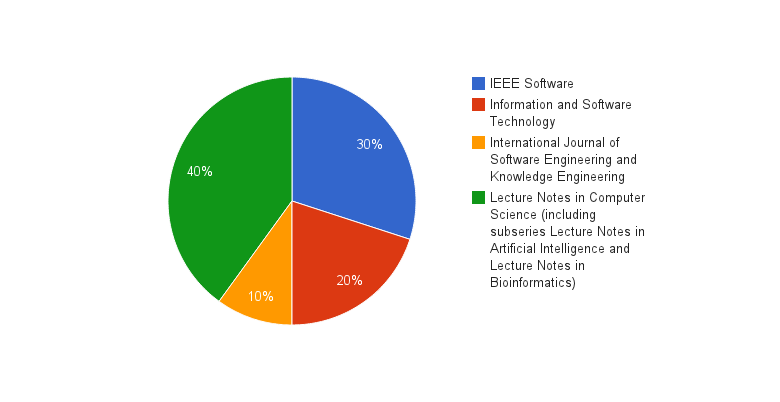
\includegraphics[width=200mm]{artikkelien_lehdet.png}
\caption{Lehdet, joissa valitut artikkelit on julkaistu.}
\label{artikkeli_lehdet_pie}
\end{figure}

Valituissa artikkeleissa on kuvattu jokin retrospektiivissä käytettävä menetelmä, joka sisältää juurisyyanalyysin käytön. Jotkin artikkeleista sisälsivät useamman menetelmän kuvauksen. Joissain tapauksissa toinen kuvattu menetelmä ei sisältänyt juurisyyanalyysiä \citep{staalhane2004root}, \citep{dingsoyr2003extending}. Nämä menetelmät on jätetty huomioimatta tässä kandidaatintyössä.

Artikkeleissa kuvatut menetelmät on jaettavissa seuraaviin yhteisiin vaiheisiin: syötteen kehittäminen, kausaalianalyysi ja parannusideoiden kehittäminen. Jako on samankaltainen, kuin mitä Lehtinen on käyttänyt artikkelissaan \citep{Lehtinen2011}. Syötteen kehittämisvaiheessa kerätään ne aiheet, joita juurisyyanalyysissä halutaan analysoida syvemmin. Kausaalianalyysivaiheessa suoritetaan varsinainen juurisyyanalyysi. Parannusideoiden kehittämisvaiheessa kehitetään kehitysideoita valituille juurisyille. Ainoastaan neljässä menetelmässä kuvatuista 12:sta menetelmästä sisältää tämän viimeisen vaiheen. Menetelmien vaiheet on kuvattu taulukossa \ref{retrovaiheet_taulukko} ja tarkemmin pohdinta-kappaleessa.

\begin{center}
\begin{longtable}{|p{3cm}|p{4cm}|p{4cm}|p{4cm}|}
\caption{Artikkelien sisältämien retrospektiivimenetelmien vaiheet}\label{retrovaiheet_taulukko}\\ \hline
  & \textbf{Syötteen kehittäminen} & \textbf{Kausaalianalyysi} & \textbf{Parannusideoiden kehittäminen} \\
\hline
\endfirsthead
\multicolumn{4}{c}%
{\tablename\ \thetable\ -- \textit{Jatkoa edelliseltä sivulta}} \\
\hline
  & \textbf{Syötteen kehittäminen} & \textbf{Kausaalianalyysi} & \textbf{Parannusideoiden kehittäminen} \\
\hline
\endhead
\hline \multicolumn{4}{r}{\textit{Jatkuu seuraavalla sivulla}} \\
\endfoot
\hline
\endlastfoot
	\textbf{\citep{kalinowski2012evidence}} & Valitaan sopiva datajoukko, luokitellaan ja priorisoidaan se (Pareto-chart) & Syy-seuraus-diagrammin, tarkemmin Fishbonen, piirtäminen mainitaan hyväksi todetuksi tavaksi tunnistaa systemaattisten ongelmien syitä. & - \\ \hline
	\textbf{\citep{Lehtinen2011}} & Fokus-ryhmän tapaaminen & 1) Kerätään syitä anonyymisti sähköpostitse. 2) Muodostetaan kerätyistä syistä suunntattu verkko 3) Brainwriting, brainstorming kokouksessa. Muodostetaan suunnattu verkko. 4) Tunnistetaan juurisyyt säköpostikyselyn avulla & Workshop, jossa parannusideoita kerätään brainwritingia yhdistettynä skeptiseen ja optimistiseen perspektiiviin. \\ \hline
	\textbf{\citep{Bjornson2009} menetelmä 1} & KJ-sessio & Fishbone (ryhmäkeskustelu) & - \\ \hline
	\textbf{\citep{Bjornson2009} menetelmä 2} & KJ-sessio & Kausaalikartan muodostaminen KJ-sessiossa & - \\ \hline
	\textbf{\citep{karlsson2006case}} & Kerätään sopiva datajoukko, uudelleenarvioidaan se ja visualisoidaan saatu data & 1) Keskustellaan visualisoidussa datassa ilmenevien ongelmien syistä. Fasilitaattori kirjoittaa keskustelusta muistiinpanoja. 2) Muistiinpanojen pohjalta luodaan taulukko, jolla löydetään eri datapisteille yhteisiä kategorioita (juurisyitä). & Kehitysideoiden kerääminen ja priorisointi \\ \hline
	\textbf{\citep{de2004learning}} & Kyselylomake 2) KJ-sessio / Semistrukturoitu haastattelu & Fishbone (ryhmäkeskustelu) & - \\ \hline
	\textbf{\citep{staalhane2004root}} & Pareto-analyysi defekteistä & 1) Fishbone (ryhmäkeskustelu) 2) Pisteytyksen avulla tunnistetaan olennaisimmat syyt (juurisyyt) & 1) Valituille syille brainstormataan kehitysideoita, jotka kootaan taulukkoon. Näistä äänestetään olennaisimmat, eli ne, jotka voitaisiin ottaa työn alle. \\ \hline
	\textbf{\citep{staalhane2003post} menetelmä 1} & 1) Projektipäälliköltä taustatietoa projektista 2) KJ-sessio ja sen tulosten priorisointi & Fishbone & Osallistujat keksivät parannusideoita Fishbone-diagrammin perusteella. Tämän jälkeen kokous. Lopulta saadaan muodostetaan lista konkreettisista parannusideoista. \\ \hline
	\textbf{\citep{staalhane2003post} menetelmä 2} & 1) Dokumenteista projektin taustatietoja 2) Strukturoitu haastattelu & Syy-seuraus-suhteita tunnistetaan haastattelun aikana (fasilitaattorilla vastuu) & Osallistujat keksivät parannusideoita lukemansa retrospektiivi-raportin perusteella. \\ \hline
	\textbf{\citep{dingsoyr2003extending}} & KJ-sessio & Fishbone &  \\ \hline
	\textbf{\citep{birk2002postmortem}} & 1) Fasilitaattori tutustuu projektiin 2) Asetetaan tavoite 3) Datankeruu ja luokittelu (KJ-sessio,  semistrukturoitu haastattelu tai fasilitoitu ryhmäkeskustelu) 4) Datan priorisointi & Fishbone (ryhmäkeskustelu) & - \\ \hline
	\textbf{\citep{card1998learning}} & 1) Valitaan sopiva datajoukko, luokitellaan ja priorisoidaan se (Pareto-chart) & Selvitetään ongelmien juurisyitä keskustelemalla ja tutkitaan löytyykö useammalla ongelmalla samoja syitä. Jos ongelman juurisyy ei löydy triviaalisti, käytetään Fishbone:a (ryhmäkeskusteluineen) apuna. & Fasilitoidun ryhmäkeskustelun avulla löydetään konkreettisia kehitysideoita. Näistä keskitytään niihin, joilla todennäköisimmiin on merkittävä vaikutus ongelmiin. \\ \hline
\end{longtable}
\end{center}

\section{Pohdinta}
Tässä kappaleessa vastataan kandidaatintyön tutkimuskysymyksiin. Ensimmäiseen tutkimuskysymykseen vastataan kuvaamalla artikkelien retrospektiivimenetelmiä. Runkona tämän osion kuvauksille toimii taulukko \ref{retrovaiheet_taulukko}.

Vertailemalla menetelmiä ja niiden vaiheita keskenään pyritään löytämään niistä tehokkaimmat ja toimivimmat piirteet. 
Vertauilun avulla ja menetelmän keveyttä arvioimalla ja sovittamalla sitä sopimaan paremmin lyhytkestoiseen ja höyhenenkevyeen ketterään retrospektiiviin vastataan toiseen tutkimuskysymykseen. Se muodostetaan lopulta synteesin avulla sille omistetussa kappaleessa. 

\subsection{Retrospektiivin eri nimitykset}
Vaikka retrospektiiveistä käyetään kirjallisuudessa lukuisia eri nimityksiä, käsittelemme niitä tässä kandidaatintyössä samalla tavalla. Pohjimmiltaan retrospektiivi \citep{AgileRetros2006}, post-mortem analyysi \citep{staalhane2003post}, postmortem analyysi \citep{de2004learning}, postmortem review \citep{dingsoyr2003extending}, process review \citep{karlsson2006case}, project review \citep{karlsson2006case}, retrospective analysis \citep{karlsson2006case}, project retrospective \citep{karlsson2006case} ja retrospective review \citep{karlsson2006case} voidaan nähdä tarkoittavan samaa asiaa.

Retrospektiivi voi olla yleinen koko analysoitavan työrupeaman kattava sessio tai sille voidaan antaa jokin tietty fokus \citep{staalhane2003post}. Fokusoituja retrospektiivejä ovat muun muassa Post-release Analysis of Requirements SElection Quality \citep{karlsson2006case} ja Defect Causal Analysis \citep{card1998learning} ja artikkelissa \citep{de2004learning} kuvattu Postmortem analyysi.

Artikkeleissa kuvatut retrospektiivit ovat eri tasoilta (lähinä projekti. myös geneerisiä tai ei tarkemmin kuvattu, milloin). TODO

\subsection{Retrospektiivien vaiheet}
Se, että artkkelien retrospektiivien menetelmien vaihejako on luonnollista tehdä niin samankaltaiseksi, kuin mitä Lehtinen on käyttänyt artikkelissaan, jossa on vertaillut eri juurisyyanalyysimenetelmiä keskenään \citep{Lehtinen2011} tuntuu mielenkiintoiselta. Voidaan nähdä, että silloin, kun juurisyyanalyysiä käytetään osana retrospektiivin menetelmää, kyseinen menetelmä ei kokonaisuudessakaan eroa juurisyyanalyysin käytöstä muussa kontekstissa. Molemmat sisältävät samanlaiset vaiheet.

Retrospektiivi käsitteenä tarkoittaa vain katsomista taakse, eli jonkin menneen tapahtuman arviointia. Ketterät menetelmätkään eivät anna sille suoraan menetelmää, vaan määrittelevät ainoastaan sen tavoitteet, joita ovat yleensä konkreettiset ehdotukset, jolla voidaan parantaa retrospektiiviin osallistuvan ryhmän työprosessia. Halutaan siis välttyä samoilta ongelmilta ja toistaa onnistumisia, joita on kohdattu. On siis vaikea tehdä eroa juurisyyanalyysiä käyttävän retrospektiivin ja muussa yhteydessä prosessinkehitystä varten pidettävän ongelmanratkaisu-juurisyyanalyysin välille.

\subsubsection{Syötteen kehittäminen}
Syötteen kehittämisvaiheessa kerätään aiheita, jotka ovat olleet retrospektiivissä käsiteltävän työrupeaman (iteraatio, projekti) kannalta merkityksellisiä. Näistä aiheista valitaan tärkeimmät, joita analysoidaan tarkemmin seuraavassa kausaalianalyysivaiheessa. Artikkelien syötteen kehittämisvaihe voidaan jakaa varsinaiseen aiheiden keräämiseen, niiden ryhmittelyyn, sekä priorisointiin.

Kuusi artikkelien kuvaamaa menetelmää \citep{birk2002postmortem}, \citep{dingsoyr2003extending}, \citep{staalhane2003post}, \citep{de2004learning}, \citep{Bjornson2009} kahdestatoista suosittelee syötteen kehittämisvaiheeseen japanilaisen etnologin, Jiro Kawakita:n mukaan nimettyä fokusoitua brainstormausmenetelmää: KJ-menetelmää \citep{dingsoyr2003extending}. Jotkin artikkeleista suosittelevat KJ-menetelmää yhtenä vaihtoehtona muiden joukossa \citep{birk2002postmortem}, \citep{staalhane2003post}, \citep{de2004learning}. Artikkeleista \citep{birk2002postmortem} on ottanut ensimmäisenä suositellut menetelmää käytettäväksi retrospektiivin syötteen kehittämiseen.

KJ-menetelmässä jokainen osallistuja saa tietyn määrän post-it -lappuja. Jokainen kirjoittaa niille sovitun määrän hyviä ja huonoja kokemuksia analysoitavasta työrupeamasta. Jokainen esittää kirjoittamansa asiat rymhälle ja asettaa laput valkotaululle. Osallistujat ryhmittelevät laput niiden aiheen mukaan ja keskustelevat niistä. \citep{birk2002postmortem}

Kaksi artikkelia kuvaa semistrukturoituja haastatteluja \citep{birk2002postmortem}, \citep{de2004learning} ja yksi strukturoituja haastatteluja \citep{staalhane2003post}. Semistrukturoidussa haastattelussa fasilitaattori valmistelee listan kysymyksiä, jotka käsittelevät retrospektiivin aihetta \citep{birk2002postmortem}. Vaikkei tekniikkaa sen tarkemmin esitellä, vaikuttaisi siltä, että niiden avulla haastattelut osallistujien kanssa pyritään ohjaamaan oikeaan suuntaan. Strukturoidussa haastattelussa suoritetaan kausaalianalyysi samalla, joten siinä kysymyksillä pyritään ohjaamaan haastattelut pohtimaan retrospektiivissä analysoitavan ongelman aiheuttajia \citep{staalhane2003post}.

Artikkelien \citep{kalinowski2012evidence}, \citep{card1998learning} kuvaamassa Defect Causal Anlaysis -menetelmässä (DCA) valitaan virheraporttitietokannasta mahdollisimman kuvaava osajoukko. Tämä osajoukko luokitellaan virhetyypin mukaan. Pääluokkien löytämiseen suositellaan Pareto-taulukon käyttämistä \citep{kalinowski2012evidence}, \citep{card1998learning}. Pareto-taulukon avulla visualisoidaan ongelmien määrä ongelmatyypeittäin rymiteltynä \citep{card1998learning}.

Moni artikkeleista suosittelee kerätyn datan priorisointia \citep{card1998learning}, \citep{birk2002postmortem}, \citep{staalhane2003post}, \citep{staalhane2004root}, \citep{karlsson2006case}. Priorisoinnin avulla voidaan valita tärkeimmät aiheet, joita käsitellään kausaalianalyysivaiheessa. DCA-menetelmää kuvaavat artikkelit \citep{kalinowski2012evidence}, \citep{card1998learning} käyttävät priorisoinnissa apuna Pareto-taulukkoa.

Artikkeli \citep{staalhane2004root} suosittelee Pareto-analyysin käyttämistä priorisointiin. Pareto-analyysi perustuu Pareto-periaatteeseen, jonka mukaan ilmiöissä usein noin 70 prosenttia seurauksista johtuu 30 prosentista syitä \citep{staalhane2004root}. 

Myös ryhmäkeskustelussa ilmenneiden prioriteettien perusteella voidaan muodostaa priorisoitu lista ongelmia \citep{staalhane2003post}. Artikkeli \citep{birk2002postmortem} ei ota kantaa siihen, miten priorisointi tapahtuu.

Artikkelissa \citep{Lehtinen2011} pidetyssä fokus-ryhmän tapaamisessa tehdään priorisointia, vaikkei sitä eksplisiittisesti mainitakaan. Kuvatussa fokus-ryhmän tapaamisessa valitaan yksi ongelma, jota otetaan käsiteltäväksi kausaalianalyysiin \citep{Lehtinen2011}.


\begin{comment}
Kalinowski
1) Ennen tapaamista
kerätään sopiva datajoukko
2) Luokitellaan
data 3) Pareto-chart:it
mainitaan hyvänä tapana
datan pääluokkien
tunnistamiseen

Lehtinen
Fokus-ryhmän tapaaminen

björnson 1\&2:
KJ

karlsson
1) Kerätään sopiva
datajoukko (valitulle
ohjelmistojulkaisulle
toteutettuja
vaatimuksia) 2) Uudelleenarvioidaan
datajoukko 3) Visualisoidaan
saatu
data

de sousa
1) Osallistujat täytt
ävät etukäteen kyselyn,
joka toimii joko
muistin virkistyksen
ä tai retrospektiivin
fokuksen löytämisessä
2) KJ-sessio / Strukturoitu
haastattelu

stålhane 2004
Tehdään Paretoanalyysi
defekteistä


(Stalhane
et al., 2003)
menetelmä 1
1) Fasilitaattori ker
ää etukäteen projektip
äälliköltä taustatietoa
projektista 2) KJsessio
3) KJ-session
tulosten priorisointi
Fishbone -

(Stalhane
et al., 2003)
menetelmä 2
1) Fasilitaattori kerää
etukäteen dokumenteista
projektin
taustatietoja 2)
Strukturoitu haastattelu
(valkotaulu ja fläppitaulu dokumentointina
ja muistin
tukena keskustelun
ajan)

dinsöyr ja hanssen 2003
KJ sessio

birk et al
1) Fasilitaattori tutustuu
projektiin,
käy mm. kaikki dokumentit
läpi. 2)
Asetetaan retrospektiiville
tavoite 3)
Kerätään positiivisia
ja negatiivisia kokemuksia
KJ-sessioilla,
semistrukturoiduilla
haastatteluilla tai
fasilitoiduilla ryhmäkeskusteluilla.

card 1998
1) Valitaan sopiva
datajoukko (voidaan
tehdä etukäteen) 2)
Luokitellaan datajoukko
(voidaan tehdä
etukäteen) 3) Tunnistetaan
olennaisimmat
datapisteet Parertochart:
in avulla
\end{comment}


\subsubsection{Kausaalianalyysi}
Kausaalianalyysivaiheessa tehdään varsinainen juurisyyanalyysi, eli analysoidaan, mistä valittu ongelma tai onnistuminen johtuu ja pyritään keksimään sille selittäviä syitä. 

Vaikka Ishikawan kalanruotodiagrammi \citep{ishikawa1990introduction} on kirjallisuudessa paljon käytetty syy-seuraus-suhteiden visualisointitapa \citep{kalinowski2012evidence}, \citep{Bjornson2009}, \citep{de2004learning}, \citep{staalhane2004root}, \citep{dingsoyr2003extending}, \citep{staalhane2003post}, \citep{birk2002postmortem}, \citep{card1998learning}, on kausaalinen kartta perustellusti osoitettu uudemmassa tutkimuksessa tehokkaammaksi visualisointitavaksi \citep{Bjornson2009}, \citep{Lehtinen2011}. 

Artikkeleissa kuvatuissa menetelmissä kahdeksan kymmenestä suosittelee kausaalianalyysiin Ishikawa diagrammin (tunnetaan myös kalanruoto, eli fishbone diagrammina) käyttöä \citep{kalinowski2012evidence}, \citep{de2004learning}, \citep{staalhane2004root}, \citep{dingsoyr2003extending}, \citep{birk2002postmortem}, \citep{card1998learning}. Kahdella artikkelilla kalanruotofiagrammi diagrammi oli kuvattu toisena menetelmänä jonkin muun rinnalla \citep{Bjornson2009}, \citep{staalhane2003post}. Kuvassa \ref{ishikawa_ex} on esimerkki kalanruotodiagrammista.

\begin{figure}[ht!]
\centering

\includegraphics[width=150mm]{ishikawa_esimerkki.png}
\caption{Esimerkki Ishikawan kalanruotodiagrammista}
\label{ishikawa_ex}
\end{figure}

Kalanruotodiagrammia käytetään syy-seuraus-suhteiden visualisointiin. Ne piirretään yleensä kollaboratiivisesti retrospektiivin osallistujien kanssa löytämään syitä postiviivisille ja negatiivisille tapahtumille \citep{birk2002postmortem}. Valkotaululle kirjoitetaan analysoitavan tapahtuman nimi ja piirretään siihen osoittava suuri nuoli \citep{Bjornson2009}. Tapahtuman syyt visualisoidaan pienemmillä nuolilla, jotka osoittavat kohti suurta nuolta \citep{Bjornson2009}. Mahdolliset alisyyt piirretään pienempinä nuolina, jotka osoittavat kohti aiheuttamaansa seurausta \citep{Bjornson2009}. Näin muodostuu kalanruotoa muistuttava kuva \citep{birk2002postmortem}.

Bj{\o}rnson on tutkimuksessaan vertaillut Ishikawan kalanruotodiagrammin käyttöä kausaaliseen karttaan \citep{Bjornson2009}. On havaittu, että kausaalianalyysivaiheessa, joka koostuu ryhmäkeskustelun lomassa muodostetusta kalanruotodiagrammista, ryhmän aktiivisuus väheni KJ-session muodossa järjestetyn syötteen keräämisvaiheeseen verrattuna \citep{Bjornson2009}, \citep{staalhane2003post}. Bj{\o}rnson kokeili KJ-session tyylistä jokaista ryhmän jäsentä osallistavaa toimintatapaa myös juurisyyanalyysivaiheessa  ja sai rohkaisevia tuloksia sen toimivuudesta \citep{Bjornson2009}. Tähän tarkoitukseen hän tarvitsi kuitenkin kalanruotodiagrammia vapaamuotoisempaa diagrammityyppiä ja päätyi kausaalisen kartan käyttöön. Kuvassa \ref{verkko_ex} on esimerkki kausaalisesta kartasta.

\begin{figure}[ht!]
\centering
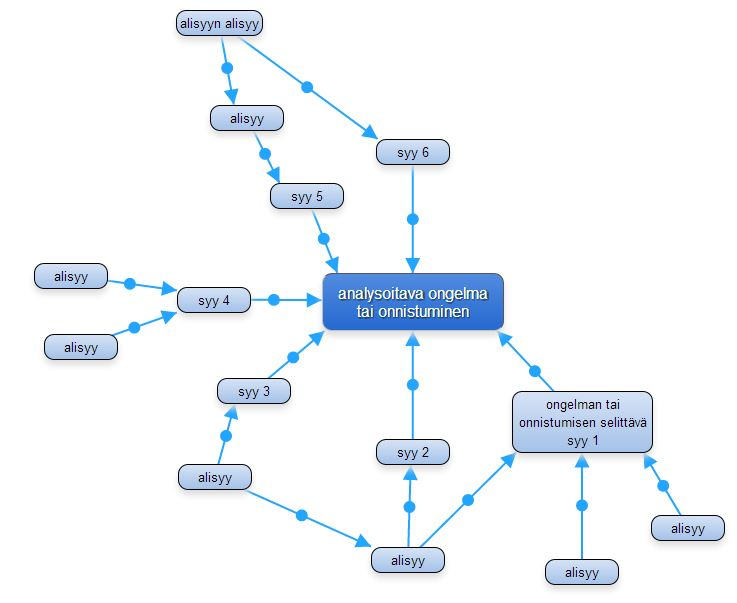
\includegraphics[width=150mm]{suunnattu_verkko_esimerkki_relaatioilla.jpg}
\caption{Esimerkki suunnatusta verkosta tai kausaalisesta kartasta (causal map)}
\label{verkko_ex}
\end{figure}

Myös Lehtinen käyttää ARCA-menetelmässään kausaalista karttaa, jota hän kutsuu suunnatuksi verkoksi \citep{Lehtinen2011}. Hän perustelee valintaa sillä, että toisin, kuin kalanruotodiagrammissa, tai muissa syy-seuraus-esitystavoissa, suunnatussa verkossa samaa syytä ei tarvitse piirtää kuin kerran, vaikka se selittäisi useampaa muuta syytä samaan aikaan \citep{Lehtinen2011}. Muun muassa kalanruotodiagrammissa useamman syyn selittävät alisyyt pitää duplikoida jokaiseen syyhyn erikseen \citep{Lehtinen2011}. 

Syyverkon Lehtinen muodostaa kahdessa eri vaiheessa: anonyymi syiden kerääminen ja kasuaalianalyysi workshop. Anonyymissä syiden keräämisessä osallistujia pyydetään lähettämään sähköpostitse ainakin viisi syytä, jotka johtavat aiemmin valittuun kohdeongelmaan. Fasilitaattori muodostaa näistä omatoimisesti suuntatun verkon, jota täydennetään kausaalianalyysi workshop:issa. Workshop:issa Lehtinen käyttää Bj{\o}rnson:in tapaan KJ-sessio tyylistä osallistavaa lähestymistapaa syyverkon täydentämiseen. \citep{Lehtinen2011}

Kausaalianalyyseistä vähiten systemaattisia lähestymistapoja kuvasivat artikkelit \citep{karlsson2006case} ja \citep{staalhane2003post}. Näissä menetelmissä syy-seuraus-suhteita löydetään ryhmäkeskustelun aikana ilman, että niitä dokumentoidaan session aikana. On fasilittaattorin vastuulla dokumentoida keskustelun aikana löytyneitä kasuaalisuuksia.

Artikkelissa \citep{card1998learning} käytetään myös vapaamuotoisen tuntuista ryhmäkeskustelua tunnistamaan ongelmien juurisyitä. Kalanruotodiagrammi piirretään vain, jos onglmien juurisyyt eivät löydy triviaalisti. Tämäkään lähestymistapa ei vaikuuta systemaattisuudellaan. Herää kysymys, minkälaisia artikkelissa kuvatut triviaalit tapaukset ovat, joihin voidaan keskustelulla, käyttämättä visualisointia apuna, tunnistaa samoja olennaisia juurisyitä, mihin muut menetelmät tarvitsevät rakenteellisen määritellyn menetelmän ja syy-seuraus-suhteiden jatkuvan visualisoinnin tehostamaan analyysiä.

Syy-seuraus-suhteiden dokumentoinnin jälkeen ainoastaan artikkelit \citep{card1998learning}, \citep{staalhane2004root}, \citep{karlsson2006case}, \citep{Lehtinen2011} valitsevat kerättyjen syiden joukosta olennaisimmat juurisyyt, joihin aikovat kehittää parannusideoita. Muissa artikkeleissa retrospektiivi loppuu syy-seuraus-suhteiden dokumentointiin.

\subsubsection{Parannusideoiden kehittäminen}

Viisi artikkelien kuvaamaa retrospektiivimenetelmää kahdestatoista kuvaa retrospektiivin päätteeksi pidettävän parannusideoiden kehittämisen \citep{card1998learning}, \citep{staalhane2003post}, \citep{staalhane2004root}, \citep{karlsson2006case}, \citep{Lehtinen2011}. Näistä artikkelit \citep{card1998learning}, \citep{staalhane2004root}, \citep{karlsson2006case}, \citep{Lehtinen2011} kehittävät parannusideoita edellisessä vaiheessa valituille tärkeimmille juurisyille. Artikkelissa \citep{staalhane2003post} parannusideoita keksitään yleisesti kausaalianalyysin perusteella.

Parannusideoiden kehittämisessä voidaan käyttää apuna fasilitoitua ryhmäkeskustelua \citep{card1998learning}, \citep{karlsson2006case}, brainstorming:ia \citep{staalhane2004root}, tai brainwriting:ia yhtdistettynä skeptiseen ja optimistiseen perspektiiviin \citep{Lehtinen2011}. Näistä kaikki menetelmät käyttävät lopuksi priorisointia tärkeimpien parannusideoiden valitsemiseksi. 

Artikkeli \citep{staalhane2003post} luottaa parannusideoiden kehittämisessä väljempään lähestymistapaan. Siinä ensimmäisessä menetelmässä osallistujilta pyydetään keksimään parannusideoita kalanruotodiagrammia tarkastellessaan. Koko retrospektiiviä käsittelevän kokouksen jälkeen muodostuu lista konkreettisista parannusideoista. Toisessa menetelmässä osallistujat keksivät parannusideat retrospektiivistä kirjoitetun raportin perusteella. \citep{staalhane2003post}

Brainwriting toteutetaan siten, että jokainen osallistuja työstää vuorollaan yhdelle valittulle juurisyylle parannusideaa ja kirjoittaa sen paperille. Tietyn ajan jälkeen jokainen antaa paperinsa vierustoverilleen. Jokainen osallistuja kontribuoi vuorollaan jokaisen juurisyyn parannusidoiden kehittämiseen. Paperit kierrätetään vielä kerran siten, että jokainen osallistuja pisteyttää kaikki kehitetyt parannusideat. Lopuksi eniten pisteitä saaneet ideat valitaan. \citep{Lehtinen2011}.

\subsubsection{Synteesi}
Vaikka kuusi artikkelin kuvaamaa menetelmää kahdestatoista pohjautuu artikkelissa \citep{birk2002postmortem} kuvattuun retrospektiivi-menetelmään on kandidaatintyön tekijän mielestä järkevää painottaa silti uudempaa tutkimusta, joka on osoitettu tätä menetelmää tuloksellisemmaksi. Uudemmalla tutkimuksella tarkoitetaan lähinnä artikkeleja \citep{Lehtinen2011} ja \citep{Bjornson2009}, sillä \citep{kalinowski2012evidence} voidaan mieltää mentelmän kuvauksen osalta ympäripyöreämmäksi verioksi aiemmasta DCA-menetelmää käsittelevästä artikkelista \citep{card1998learning}.

Bj{o}rnsonin artikkelia vanhemmat artikkelit käyttävät joko epäsystemaattisen tuntuisia menetelmiä, kuten \citep{karlsson2006case}, \citep{staalhane2003post} ja kausaalianalyysin osalta \citep{card1998learning}, tai perustuvat artikkelin \citep{birk2002postmortem} kuvaamaan retrospektiivimenetelmään.

Kuitenkin on otettava huomioon, ettei yksikään artikkeleissa kuvatuista menetelmistä kuvaa suoraan ketterää retrospektiiviä, vaan suuremman mittakaavan ja enemmän aikaa vieviä retrospektiivejä, kuten projektin jälkeen pidettäviä retrospektiivejä. (tähän kappaleeseen viitteet) Artikkelien kuvaamista menetelmistä valitaan siis parhaat palat, minkä jälkeen niitä skaalataan kevyemmiksi ja siten paremmin sopiviksi käytännöiksi ketterään retrospektiiviin.

Syötteen kehittämisvaiheeseen valitaan KJ-menetelmä, koska se on monissa artikkeleissa käytetty syötteen kehittämismenetelmä ja parantaa Bj{o}rnsonin mukaan retrospektiivin osallistujien aktiivisuutta \citep{Bjornson2009}. KJ-session jälkeen valitsemme ehdotetuista positiivisista ja negatiivisista kokemuksista olennaisimmat priorisoimalla ehdotukset

Pareto-analyysi \citep{staalhane2004root}, Pareto-taulukko \citep{card1998learning}, \citep{kalinowksi2012evidence} tai brainwriting \citep{Lehtinen2011} olisivat kaikki hyviä varmoja tapoja tehdä priorisointi oikein perustein. Ne ovat kaikki kuitenkin myös aikaa vieviä menetelmiä. Myös ryhmäkeskustelu \citep{staalhane2003post} voi viedä paljon aikaa. Perinteinen käsiäänestys voisi olla tehokas tapa hoitaa priorisointi. Siinä käytäisiin ehdotetut kokemus-luokat läpi ja jokainen saisi äänestää niistä yhtä suosikikseen. Eniten ääniä saanut luokka valittaisiin kausaalianalyysiin.

Kausaalianalyysiin valitaan menetelmäksi KJ-menetelmä ja syy-seuraus-suhteiden visualisointiin suunnattu verkko, joita suositellaan artikkeleissa \citep{Lehtinen2011}, \citep{Bjornson2009}. Kausaalianalyysin päätteeksi tärkeimmät juurisyyt valitaan käsiäänestyksellä.



\subsection{Kandidaatintyön validiteetti ja sen uhkat}
Systemaattisen kirjallisuuskatsauksen validiteettiin vaikuttaa luonnollisesti se, että sen on suurimmalta osin suorittanut yksi henkilö (kandidaatintyön kirjoittaja) oman arviokykynsä mukaan. Kandidaatityön ohjaaja on auttanut kandidaatintyön tekijää esimerkiksi hakusanojen valinnassa, mutta suorittava työ, kuten artikkeline arviointi ja rajaus on ollut kandidaatintyön tekijän vastuulla. On mahdollista, että joitain olennaisia artikkeleja karsiutui väärin perustein pois, koska abstraktia oli tulkittiin väärin. On myös todennäköistä, ettei valittuhakutermimme saavuttanut kaikkia olennaisia artikkeleja, mikäli ne eivät sisältäneet käytettyjä hakusanoja.

Silti on perusteltua pitää suoritettua systemaattista kirjallisuuskatsausta huomattavasti luotettavampana ja tieteellisempänä tutkimusmenetelmänä, kuin tyypillinen sattumanvaraisten, erilaisten hakusanojen kokeilu eri hakukoneissa ja niiden hakutuloksista mielivaltaisin perustein valittujen artikkelien lukeminen. Tarkat ja hyvin dokumentoidut artikkelien valintakriteerit ja muut systemaattisen kirjallisuuskatsauksen eri vaiheet tekevät tutkimuksesta helposti toistettavan ja tarkistettavan. Tämä parantaa tehdyn tutkimuksen validiteettia huomattavsti.

Lisäksi aineistohaun rajaaminen ennalta karsittuun joukkoon (Scopus-hakukone) ja sieltä pelkkien tieteellisten artikkelien, jotka käyvät julkaisuvaiheessa tiukan karsintaprosessin, valinta parantaa käsitellyn aineiston luotettavuutta.

\section{Yhteenveto}
